\documentclass[1p,16pt]{elsarticle}
\makeatletter
\def\ps@pprintTitle{%
\let\@oddhead\@empty
\let\@evenhead\@empty
 \def\@oddfoot{}%
 \let\@evenfoot\@oddfoot}
\makeatother

%% Use the option review to obtain double line spacing
%% \documentclass[authoryear,preprint,review,12pt]{elsarticle}

%% Use the options 1p,twocolumn; 3p; 3p,twocolumn; 5p; or 5p,twocolumn
%% for a journal layout:
%% \documentclass[final,1p,times]{elsarticle}
%% \documentclass[final,1p,times,twocolumn]{elsarticle}
%% \documentclass[final,3p,times]{elsarticle}
%% \documentclass[final,3p,times,twocolumn]{elsarticle}
%% \documentclass[final,5p,times]{elsarticle}
%% \documentclass[final,5p,times,twocolumn]{elsarticle}

%% For including figures, graphicx.sty has been loaded in
%% elsarticle.cls. If you prefer to use the old commands
%% please give \usepackage{epsfig}

%% The amssymb package provides various useful mathematical symbols
\usepackage{amssymb}
\usepackage{amsmath}
\usepackage{graphicx}
\graphicspath{{./figures/}}
\usepackage[colorlinks]{hyperref}
\hypersetup{citecolor=DeepPink4}
\hypersetup{linkcolor=DarkRed}
\hypersetup{urlcolor=DarkBlue}
\usepackage{hyperref}
\usepackage{subcaption}
\usepackage{minted}

%% The amsthm package provides extended theorem environments
%% \usepackage{amsthm}

%% The lineno packages adds line numbers. Start line numbering with
%% \begin{linenumbers}, end it with \end{linenumbers}. Or switch it on
%% for the whole article with \linenumbers.
%% \usepackage{lineno}

\journal{Hardware and Embedded Systems Security}

\begin{document}

\begin{frontmatter}

%% Title, authors and addresses

%% use the tnoteref command within \title for footnotes;
%% use the tnotetext command for theassociated footnote;
%% use the fnref command within \author or \address for footnotes;
%% use the fntext command for theassociated footnote;
%% use the corref command within \author for corresponding author footnotes;
%% use the cortext command for theassociated footnote;
%% use the ead command for the email address,
%% and the form \ead[url] for the home page:
%% \title{Title\tnoteref{label1}}
%% \tnotetext[label1]{}
%% \author{Name\corref{cor1}\fnref{label2}}
%% \ead{email address}
%% \ead[url]{home page}
%% \fntext[label2]{}
%% \cortext[cor1]{}
%% \address{Address\fnref{label3}}
%% \fntext[label3]{}

\title{Assignment 2: Side-Channel Analysis and Fault Injection}

%% use optional labels to link authors explicitly to addresses:
%% \author[label1,label2]{}
%% \address[label1]{}
%% \address[label2]{}

\author{Amar Lakshya (AXX945), Calvin Menezes (CXM1010)}

\address{School of Computer Science, University of Birmingham}

% \begin{abstract}
%
% \end{abstract}
%
% \begin{keyword}
% %% keywords here, in the form: keyword \sep keyword
% %% PACS codes here, in the form: \PACS code \sep code
% %% MSC codes here, in the form: \MSC code \sep code
% %% or \MSC[2008] code \sep code (2000 is the default)
%
% \end{keyword}
%
\end{frontmatter}

%% \linenumbers

%% main text
\section{Task1}
% \label{Task1}
The average number of cycles per execution of the exponentiation for e = 17 is:
\textbf{9,224,516} cycles.
\\
First, we change the exponent bit form 17 to 12 (1100) so that we have a 50\%
distribution of 1s and 0s as required by the problem and the recorded value
through the program is: \textbf{7,365,416} cycles.\\

Let $C_{4}$ be the cycles for a 4-bit exponent exponentiation with 50\% distribution of 1s and 0s.\\
Let $C_{1024}$ be the cycles for a 1024-bit exponent exponentiation with 50\% distribution of 1s and 0s.\\
\begin{align}
	C_4 &= 7365416 \\
	C_{1024} &=  C_4 * 256 (1024 = 4 * 256) \\
	C_{1024} &= 7365416 * 256 \\
	C_{1024} &= 1885546496
\end{align}

Therefore, the extrapolated cycles for a 1024-bit exponent exponentiation where 50\% of bits are 1 is:
\textbf{1,885,546,496} cycles.
\section{Task2}
% \label{Task2}

\subsection{Oscilloscope Capture}%
\label{sub:oscilloscope_capture}
The image of the RSA operations can be seen below:
\begin{figure}[H]
	\centering
    \centerline{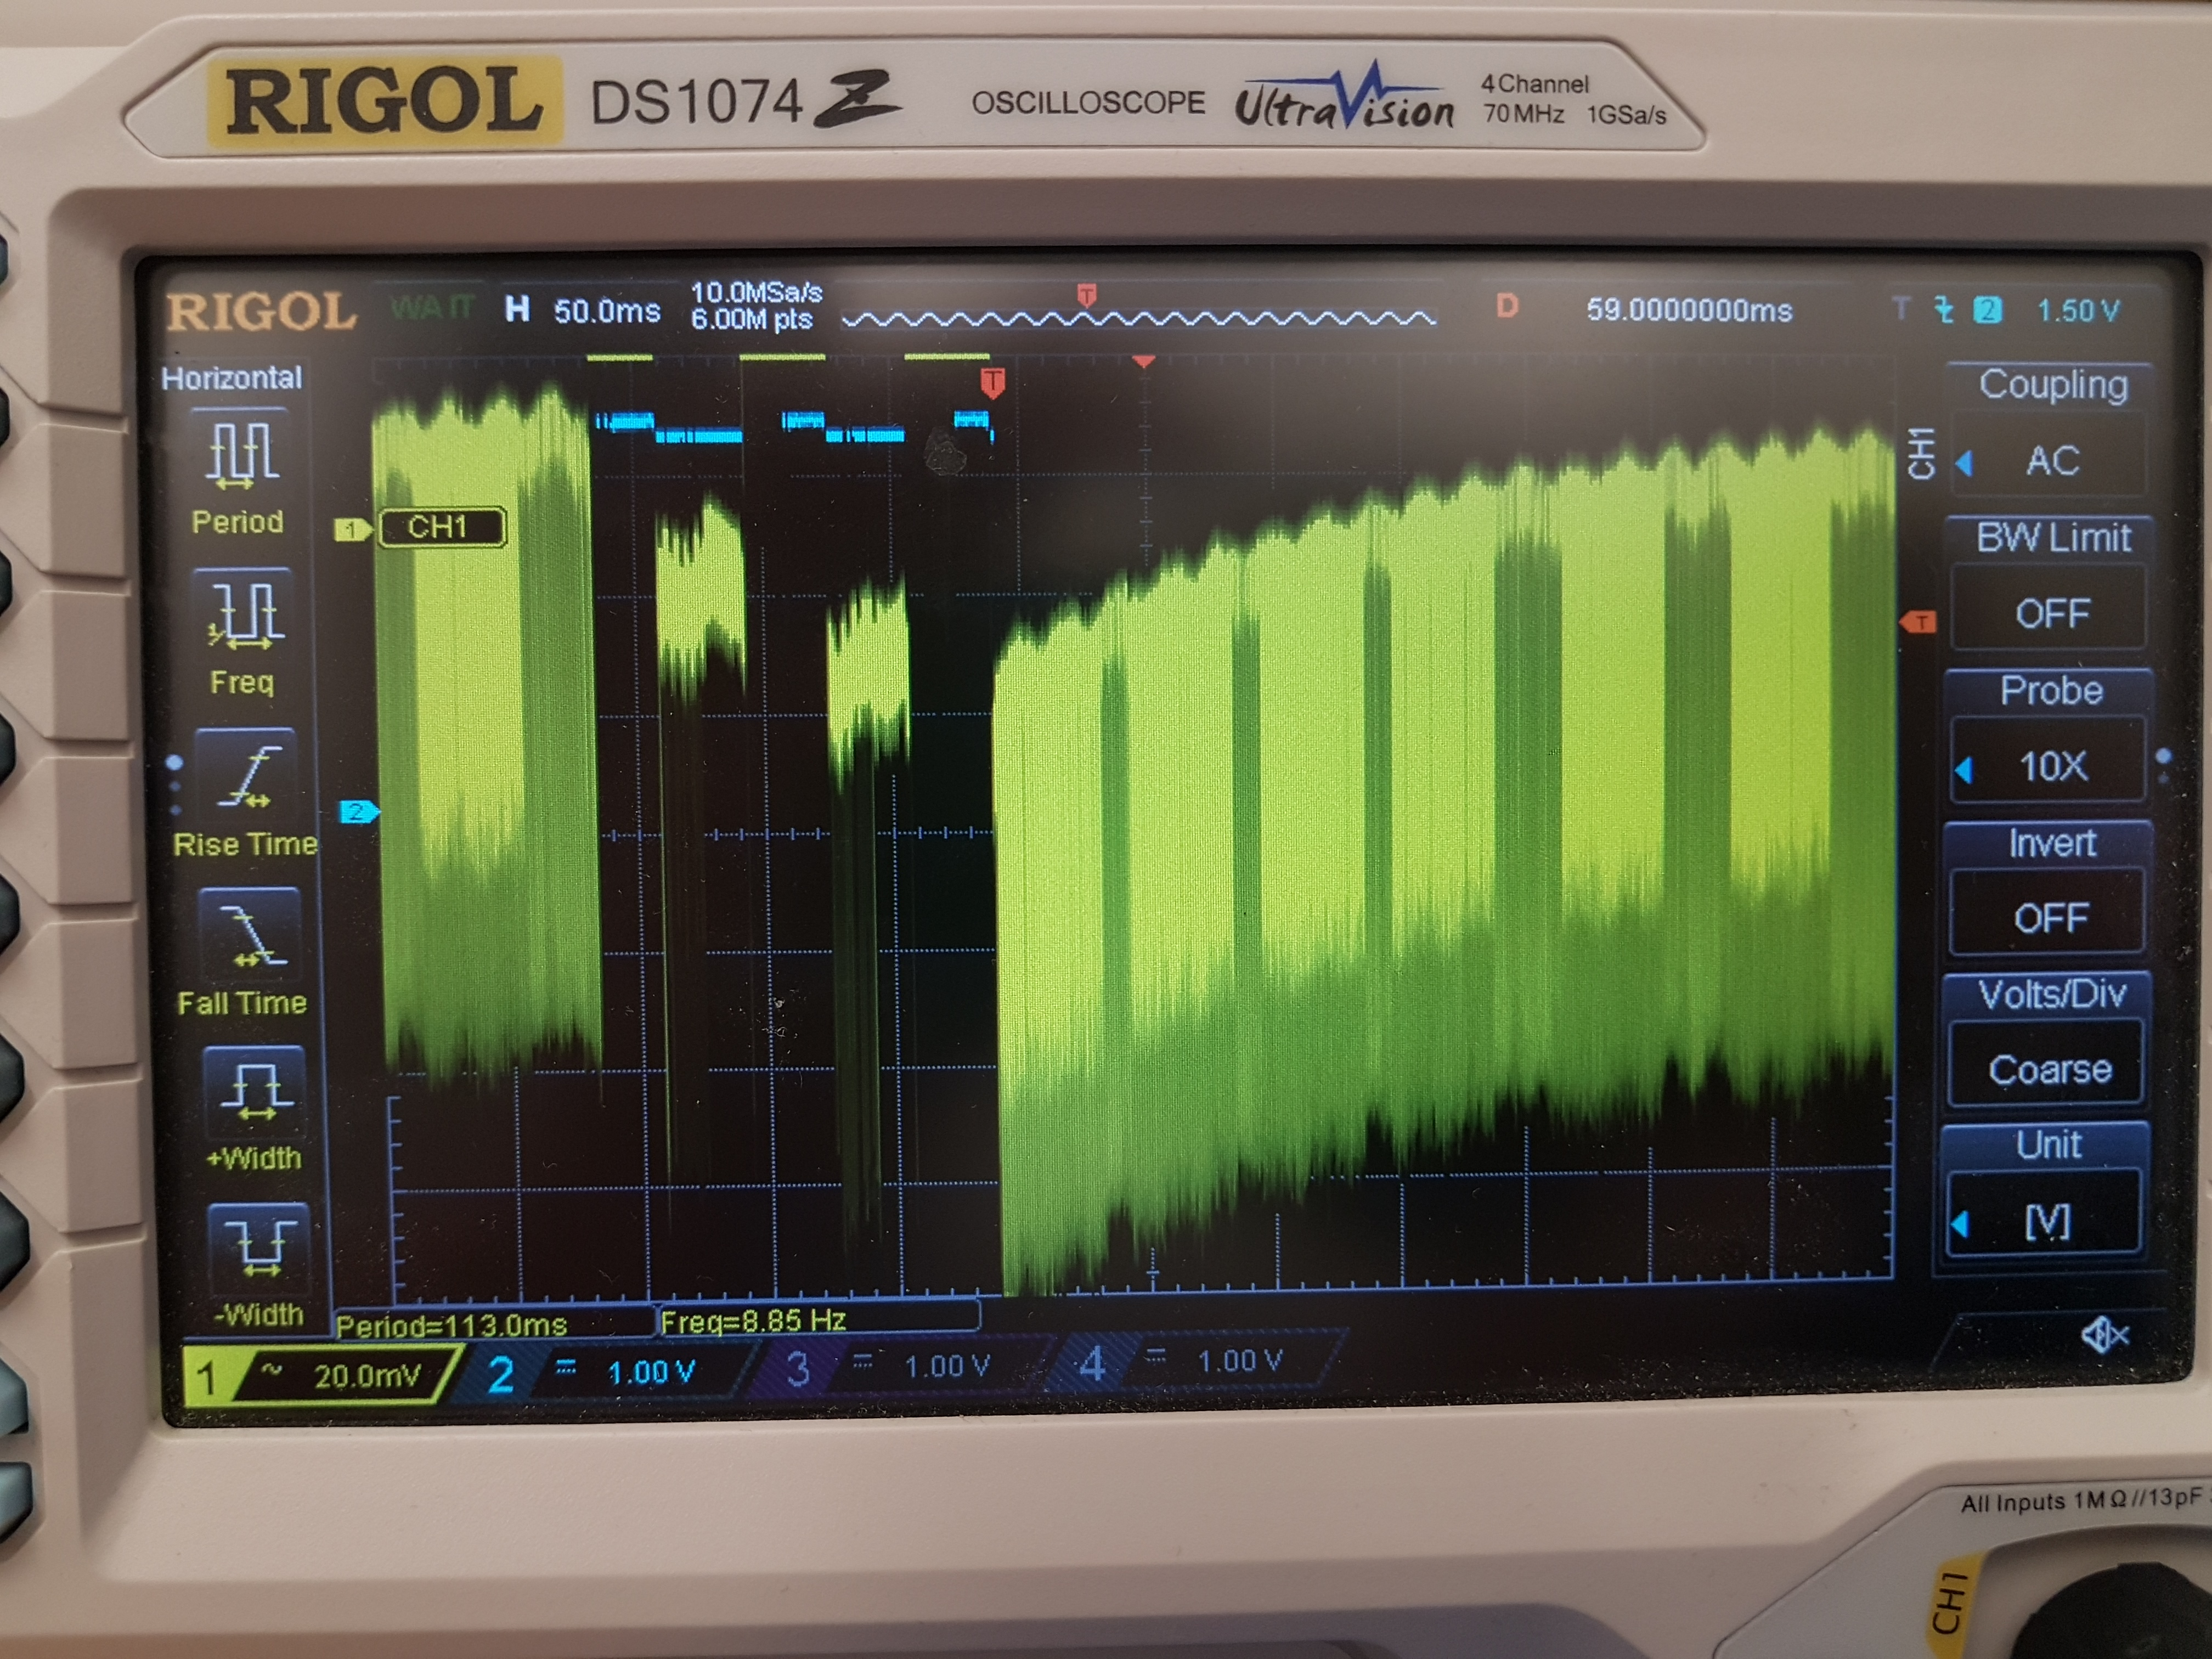
\includegraphics[width=7cm]{oscilloscope}}
    \caption{The picture of oscilloscope showing the first 6 operations of RSA}\label{fig:oscilloscope}
\end{figure}

\subsection{Manual Extraction}%
\label{sub:manual_extraction}

\begin{figure}[H]
	\centering
    \centerline{\includegraphics[width=10cm]{manual_extraction}}
    \caption{Superimposed picture showing operations as seen in the trace}\label{fig:manual_extraction}
\end{figure}
\begin{itemize}

\item Based on the square-and-multiply (SaM) algorithm, the for-loop contains a square (S) operation that takes place in every iteration and a multiply (M) operation that is done only when the current exponent bit is 1.

\item The initial bit of the exponent is always 1 and the loop starts from the 2nd bit onwards (Left to right).

\item The screenshot above from an oscilloscope shows variation in power consumption as the algorithm runs.

\item The thinner lines plotted indicate a square operation and the thicker lines indicate squaring followed with multiplication.

\item The sequence of operations from the graph are S, S, S, SM, SM, SM that translates to the bits being 0,0,0, 1, 1, 1.

\item Therefore, the upper six bits of the exponent e are 100011.

\end{itemize}


\subsection{Acquired Trace}%
\label{sub:acquired_trace}

\begin{figure}[H]
	\centering
    \centerline{\includegraphics[width=10cm]{trace_plot}}
    \caption{Graph of the acquire trace in full scale}\label{fig:acquired_trace}
\end{figure}

The graph of the acquired trace can be found above and
the program file \textit{task2.3.py} contains the program.

\subsection{SPA}%
\label{sub:spa}

The following is the output of the submitted \textit{task2.4.py} program:
\begin{minted}{bash}
Iterating through 520000 sample points from trace_filtered.dat
Analyzing waveform... ... ...

----- Exponent extracted -----

        Binary: 1110 1111 1110 1010 1001 1001 0000 0111
		Hex: efea9907
\end{minted}

\section{Task3}
% \label{Task3}

\subsection{Overlapping Traces}%
\label{sub:overlapping_traces}


\begin{figure}[H]
	\centering
    \centerline{\includegraphics[width=10cm]{traces_plot}}
    \caption{Graph of superimposed 10 traces}\label{fig:traces_plot}
\end{figure}

The plot of the first 10 traces can be seen above.
\par
The program file \textit{task3.py} contains the program for the task.
The corresponding output can be seen below:
\begin{minted}{bash}
byte value for trace 0: D8
byte value for trace 1: E8
byte value for trace 2: 42
byte value for trace 3: 3D
byte value for trace 4: 96
byte value for trace 5: E5
byte value for trace 6: CB
byte value for trace 7: 0B
byte value for trace 8: 1F
byte value for trace 9: 33
\end{minted}

\subsection{AES XOR}%
\label{ssub:aes_xor}
The following function implements the required functionality (the complete program can be found in the submitted zip):

\begin{minted}{python}
def AES_XOR(x, k_prime):
    return SBOX[x ^ k_prime]
\end{minted}

\subsection{Significant Bit}%
\label{sub:significant_bit}
The method to extract the \textit{MSB} involves two steps where we first convert an \textit{integer}
to a \textit{bit-field} and then we get the first element of the \textit{bit-field}.
The following is an implementation of the function in \textit{python}:
\begin{minted}{python}
def int_to_bits(n):
    return [n >> i & 1 for i in range(BIT_SIZE-1,-1,-1)]

def MSB(n):
    return int_to_bits(n)[0]
\end{minted}

\subsection{DPA}%
\label{sub:dpa}

\begin{figure}[H]
	\centering
    \centerline{\includegraphics[width=10cm]{peaks_plot}}
    \caption{Graph of superimposed difference-of-means}\label{fig:peaks_plot}
\end{figure}

The submitted program file \textit{task3.4.py} contains the program to produce the overlapping graphs
of all difference-of-means curves as seen above and the zoomed-in part
showing the candidate key $K10=7$ can be seen below.

\begin{figure}[H]
	\centering
    \centerline{\includegraphics[width=10cm]{peak_plot}}
    \caption{Graph of zoomed-in part of difference-of-means}\label{fig:peak_plot}
\end{figure}

\section{Task4}
% \label{sub:task4}

\subsection{Fault Injection on RSA-CRT}%
\label{sub:fault_injection_on_rsa_crt}
From the given values
$n=91, e=5, S=48, \overline{S}=35, x=55$
we calculate the valid signature $y$ by:
\begin{align}
	y &= x^e \mod n \\
	y &= 55^5 \mod 91 \\
	y & = 48
\end{align}

\subsubsection{Using Bellcore Method}%
\label{sub:ballcore_method}
The bellcore method gives factor $q$ by:
\begin{align}
	q &= \gcd(S - \overline{S}, n) \\
	q &= \gcd(48 - 35, 91) \\
	q &= \gcd(13, 91) \\
	q &= 13
\end{align}

we know $n = p * q$ therefore factor $p$ is:
\begin{align}
	p &= n / q \\
	p &= 91 / 13 \\
	p &= 7
\end{align}


\subsubsection{Using Lenstra Method}%
\label{sub:lenstra_method}
The Lenstra method gives factor $q$ by:
\begin{align}
	q &= \gcd(\overline{y}^e - x, n) \\
\end{align}

From eq 1, we know that $y=48$ and since
$\overline{y} = y, \overline{y} = 48$, therefore

\begin{align}
	q &= \gcd(48^5 - 55, 91) \\
	q &= \gcd(48 - 55, 91) \\
	q &= \gcd(7, 91) \\
	q &= 7
\end{align}

we know $n = p * q$ therefore factor $p$ is:

\begin{align}
	p &= n / q \\
	p &= 91 / 7 \\
	p &= 13
\end{align}

The major advantage of Lenstra method is that only the faulty value $\overline{S}$ needs to be known.



\subsection{Counter Measures}%
\label{sub:counter_measures}

\subsubsection{Difference between Detection based and Algorithmic}%
\label{sub:difference_between_detection_based_and_algorithmic}
\begin{itemize}
	\item Detection-based countermeasures are based in detecting faults through hardware or software properties
		of faults while Algorithmic take help of specific algorithmic patterns and monitor changes in those
		patterns caused by faults.
	\item Since Algorithmic countermeasures can use techniques like time randomization, they are much harder
		to inject faults against.
\end{itemize}

\subsubsection{RSA-CRT Countermeasures}%
\label{sub:rsa_crt_countermeasures}
\begin{itemize}
	\item Detection-based countermeasures
		\begin{itemize}
			\item \textbf{TODO}
		\end{itemize}
	\item Algorithmic countermeasures
		\begin{itemize}
			\item A simple countermeasure could be to do verification of the signature before and after
				RSA-CRT using Hashes.
			\item \textbf{TODO}
		\end{itemize}
\end{itemize}

\subsubsection{SPA Prevention}%
\label{sub:spa_prevention}
There a number of countermeasures that can be taken to prevent the SPA attack:
\begin{itemize}
	\item The Square and Always Multiply Algorithm can be used to conditionally throw away the result
		so that there's less contrast in the acquired power trace.
	\item Noise Addition or Signal Reduction can be implemented on the signal to reduce the SNR
	\item Balancing power consumption requires a lot of changes in hardware that create redundant circuits
		and is therefore not a preferred countermeasure.
\end{itemize}

\subsubsection{Time Randomization}%
\label{ssub:time_randomization}
\begin{itemize}
	\item In Both Fault Injections models namely \textit{Flip-Bit} and \textit{Stuck-at},
		the faults are injected in order to alter the normal control flow of a program
		and since the instructions in a control flow are dependent on time, Time Randomization
		makes these injections to work.
	\item In Side-Channel attacks focus on recovering secrets through analysis of the Runtime.
		Since the Runtime of a program is based on time, Time randomization makes these attacks
		also harder to work.
\end{itemize}

\subsubsection{DPA Effects}%
\label{ssub:dpa_effects}
\begin{itemize}
	\item Increasing the amplitude noise decreases the SNR and therefore each power trace
		will have lesser amount of signal and a greater number of traces will be required.
	\item If the attacker can acquire infinitely many traces then increasing noise below a certain
		point (after which the signal is no longer traceable)
		will not be a suitable countermeasure. However under a finite number of traces,
		this technique can function as an effective countermeasure.
\end{itemize}


%% The Appendices part is started with the command \appendix;
%% appendix sections are then done as normal sections
%% \appendix

%% \section{}
%% \label{}

%% If you have bibdatabase file and want bibtex to generate the
%% bibitems, please use
%%
% \bibliographystyle{elsarticle-num}
% \bibliography{bibliography}
%

%% else use the following coding to input the bibitems directly in the
%% TeX file.

% \begin{thebibliography}{00}
%
% %% Text of bibliographic item%
% \end{thebibliography}
\end{document}
\endinput
%%
%% End of file `elsarticle-template-num.tex'.
